\chapter{Analyse de la base de données d’IMPatienT par IA Explicable (xAI)}

\section{Contexte}
La création d'un vocabulaire standard décrivant les observations (termes) faites lors de la biopsie musculaire a permis grâce à \gls{impatient} la numérisation de 89 rapports de biopsie de patients atteints de \gls{mc}. Ce tableau de données peut servir de jeu de données pour l'entraînement de modèles \gls{ml} traditionnels pour en évaluer les performances et les comparer aux modèles explicables. C'est précisément l'objet de cette analyse.
\section{Contenu de la base de données}
Chacun des 89 rapports d'histologie ont été numérisés à la main en annotant via \gls{impatient} chacun des termes du vocabulaire entre: absence du terme (0), présence (suivant 4 gradations de quantité de 0.25 à 1) ou absence d'information (N/A).  Cette procédure a permis d'obtenir une matrice numérique de taille (89,175) où les 175 colonnes représentent les 175 termes du vocabulaire standard. De plus, pour chacun des 89 rapports un certain nombre de méta-données ont été enregistrées en plus tel que: l'âge, le numéro de biopsie, le muscle, le diagnostic final, l'identifiant de la biopsie, l'identifiant unique du patient.
\subsection{Analyse statistique exploratoire}
Dans un premier temps j'ai réalisé une analyse statistique exploratoire de ce jeu de données (fig. \ref{fig:impatient_eda}). Ainsi grâce à \gls{impatient} j'ai généré plusieurs visualisation dont des histogrammes, des matrices de corrélations, des tableau de fréquences et des matrice de confusions pour évaluer la méthode \gls{boqa}.  On observe dans notre jeu de données une majorité de patient adultes (49 sur 89). Au niveau des gènes, les gènes TTN, NEB, RYR1 et MYH7 sont les plus souvent responsables de la maladie (40 sur 89). Au niveau diagnostic, les \gls{com} et les \gls{nm} sont les plus communes (28 et 25). Ensuite il y a un grand groupe de patients sans diagnostic clairement établis (23) puis un groupe plus petit de patients à \gls{cnm} (10). Les tableaux des termes les plus fréquents par gène et par diagnostic font ressortir des termes attendues tels que une forte fréquence de bâtonnets sombres dans les \gls{nm}, de noyaux centralisés dans les \gls{cnm} et de cores dans les \gls{com}.
\begin{figure}[htbp]
  \centering
  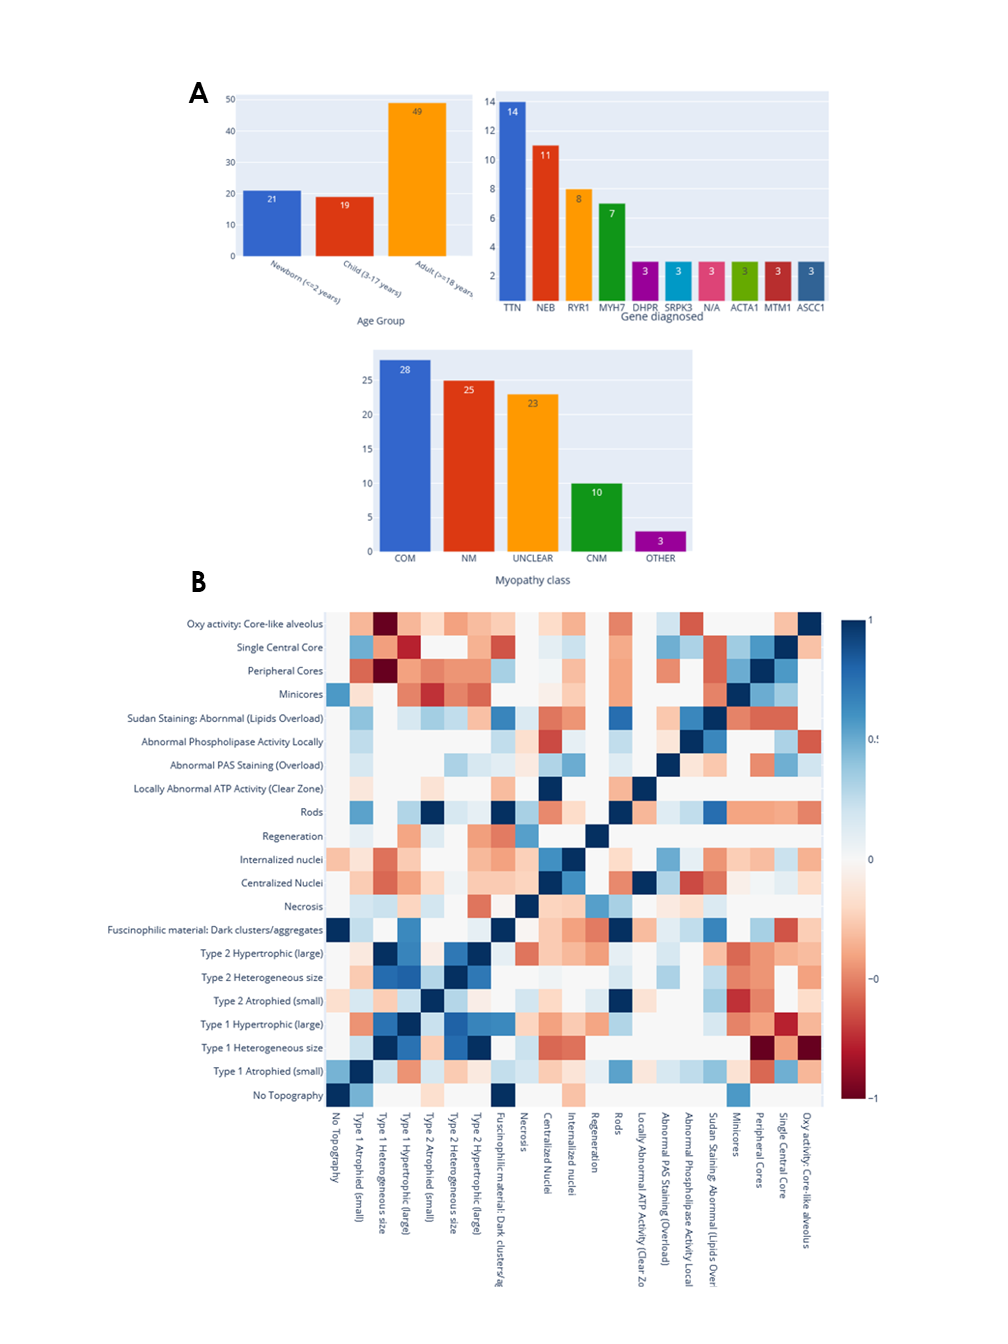
\includegraphics[width=0.98\textwidth]{figures/impatient_explo.png}
  \caption[Analyse statistique exploratoire IMPatienT]{Analyse statistique exploratoire de la base de données IMPatienT. (A) Histogrammes de répartition des patients, (B) Matrice de corrélation des termes du vocabulaire standard.}
  \label{fig:impatient_eda}
\end{figure}
\section{Pipeline de Machine-Learning Streamline}
Nous avons voulu évaluer si il était possible de prédire le diagnostic des patients via des techniques classification par algorithmes de \gls{ml} traditionnels. Pour cela nous avons utilisé et modifié le pipeline Streamline (\cite{urbanowicz_streamline_2022}), développé par \textit{Ryan J. Urbanowicz}, créateur aussi d'un algorithme de classification explicable (de type \gls{lcs})  nommé Exstracs 2.0 (\cite{urbanowicz_exstracs_2015}).
Le pipeline Streamline permet d'entraîner, d'optimiser et de comparer 11 algorithmes traditionnels de \gls{ml} sur un même jeu de données. Ce pipeline est développé pour de la classification binaire, j'ai donc procéder à des modifications pour le rendre compatible avec des tâches de classification multi-classe (prédiction de diagnostic entre les \gls{nm}, \gls{com} et les \gls{cnm}).
\section{Résultats d'analyse}
L'utilisation de Streamline nous a permis de comparer 11 algorithmes de \gls{ml} pour la classification de données biomédicales (table \ref{table:ml_metrics}). Parmi ces 11 algorithmes, 9 ont montré des performances similaires, avec une exactitude de classification se situant entre 0,77 et 0,83. Cependant, les algorithmes eLCS et xLCS ont obtenu des performances nettement inférieures, avec une exactitude de classification de 0,32 et 0,34 respectivement (performances quasi aléatoire). Ces résultats se perçoivent aussi en observant la courbe ROC (fig. \ref{fig:roc_curve}).
\begin{figure}[htbp]
  \centering
  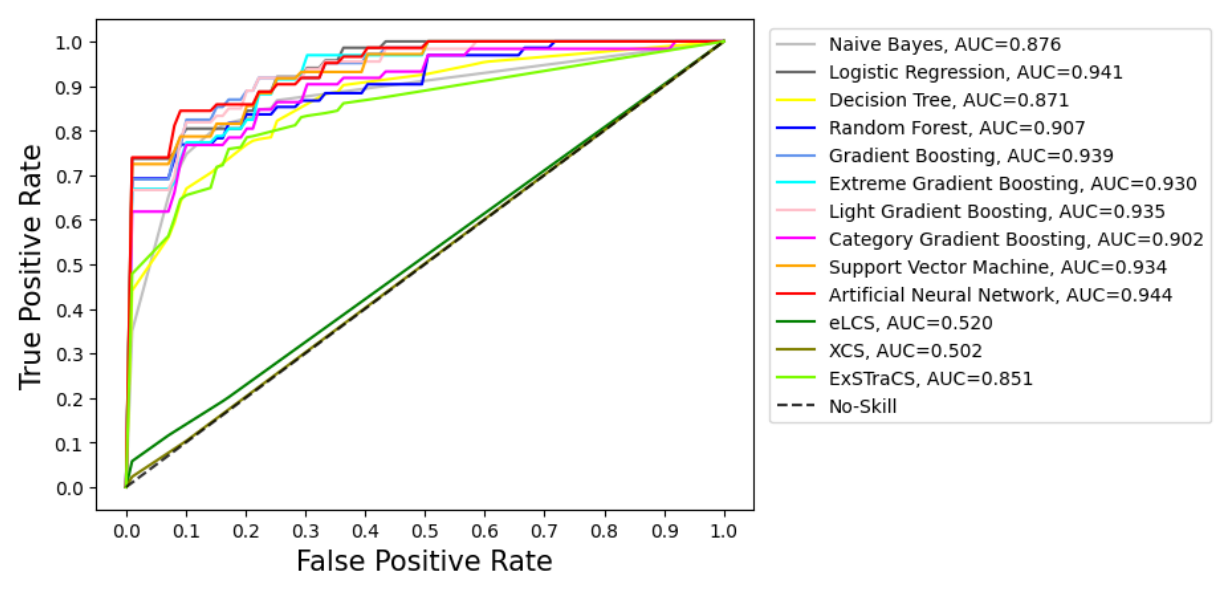
\includegraphics[width=1\textwidth]{figures/roc_streamline.png}
  \caption[Comparaison des courbes ROC]{Comparaison des courbes ROC des 11 algorithmes comparés.}
  \label{fig:roc_curve}
\end{figure}
\begin{table}[htbp]
\centering
\begin{tabular}{lcccc}
\hline
Algorithme & Exactitude Pondérée & Exactitude & Matthew Corr. Coeff. & Spécificité  \\
\hline
Naive Bayesienne & 0.77 & 0.82 & 0.73 & 0.91 \\
Regession Logistique & 0.75 & 0.79 & 0.69 & 0.89 \\
Arbre de décision & 0.72 & 0.77 & 0.62 & 0.86 \\
Random Forest & 0.74 & 0.77 & 0.67 & 0.89 \\
Boosting & 0.81 & 0.82 & \textbf{0.75} & 0.91 \\
XGBoost & 0.72 & 0.77 & 0.66 & 0.89 \\
LGB & 0.73 & 0.80 & 0.71 & 0.90 \\
Cat-Boost & 0.71 & 0.77 & 0.66 & 0.89 \\
SVM & \textbf{0.83} & 0.80 & 0.74 & 0.90 \\
Perceptron & 0.74 & \textbf{0.83} & 0.74 & \textbf{0.92 }\\
eLCS & 0.32 & 0.38 & 0.05 & 0.69 \\
XCS & 0.33 & 0.46 & 0.04 & 0.73 \\
ExSTraCS & 0.68 & 0.77 & 0.65 & 0.89 \\
\hline
\end{tabular}
\caption{Comparaison des performances des modèles (moyenne sur 10 CV)}
\label{table:ml_metrics}
\end{table}        
L'algorithme \gls{svm} s'est révélé être le meilleur algorithme en terme d'exactitude pondérée. En revanche, l'algorithme de système de classeur ExSTraCS 2.0, qui présente l'avantage d'être très explicable, a affiché une performance légèrement inférieure, avec une exactitude de classification de 0,77 (et de 0,68 pour l'exactitude pondérée). Il est intéressant de noter que l'algorithme de classification naïve bayésienne, qui est à la fois simple et par nature explicable, a obtenu des performances similaires à celles de la SVM, tout en ayant un temps d'entraînement faible de 22 secondes en raison de sa simplicité et de l'absence d'hyper-paramètre à optimiser (table \ref{tab:pipeline_times}). A titre de comparaison, le \gls{lcs} ExSTraCS a nécessité un temps d'entraînement de  9 minutes, et ceci sans phase d'optimisation des hyper-paramètres.
\begin{table}[htbp]
    \centering
    \begin{tabular}{lr}
        \toprule
        Algorithme & Temps d'optimisation et d'entraînement (sec) \\
        \midrule
        Naive Bayesienne & 22.89 \\
        Regession Logistique & 61.82 \\
        Arbre de décision & 29.6 \\
        Random Forest & 3325.78 \\
        Boosting & 3078.92 \\
        XGBoost & 1345.9 \\
        LGBoost & 329.61 \\
        Cat-Boost & 6664.66 \\
        SVM & 39.04 \\
        Perceptron & 1391.7 \\
        eLCS & 1909.32 \\
        XCS & 1832.16 \\
        ExSTraCS & 534.56 \\
        \bottomrule
    \end{tabular}
    \caption{Temps d'optimisation et d'entraînement des algorithmes}
    \label{tab:pipeline_times}
\end{table}
\begin{figure}[htbp]
  \centering
  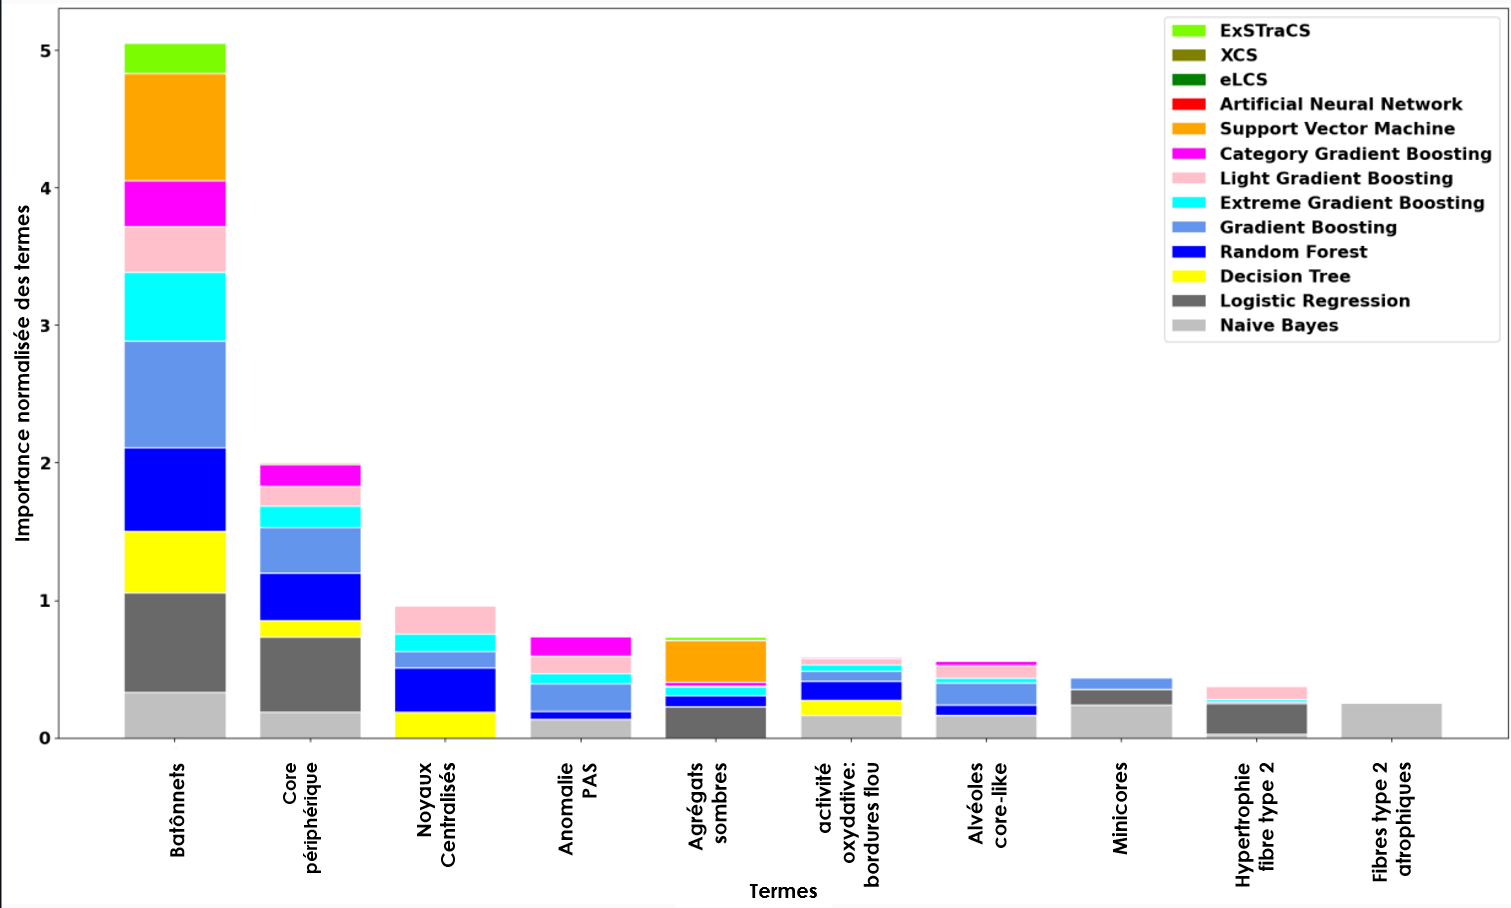
\includegraphics[width=1\textwidth]{figures/feature_importance.png}
  \caption[Histogramme des 10 termes les plus déterminants pour la classification]{Histogramme des 10 termes les plus déterminants pour la classification}
  \label{fig:feautre_importance}
\end{figure}
L'histogramme montrant les 10 termes les plus importants pour la classification dans l'ensemble des algorithmes (fig. \ref{fig:feautre_importance}) met en évidence des termes attendu comme le présence de bâtonnet, de core ou de noyaux centralisés pour faire la différence entre \gls{nm}, \gls{com} et \gls{cnm} avec un poids très important pour la présence de bâtonnets. Mais on observe aussi la présence de critère moins attendu comme la présence d'anomalie au marquage PAS et l'hypertrophie ou atrophie des fibres de type 2.
L'ensemble de ces résultats suggèrent que la taille et l'hétérogénéité du jeu de données pourraient être insuffisantes pour permettre une comparaison des algorithmes. Sur notre jeu de donnée, il semblerait que l'utilisation d'algorithmes simples comme la méthode naïve bayésienne soit à privilégier pour sa triple efficacité en terme de performances, explicabilité et coût en puissance de calcul.  Il est possible que l'utilisation d'un ensemble de données plus important, c'est à dire contenant plus de compte-rendus de biopsie, et homogène permettrait une meilleure évaluation des performances de ces algorithmes et, par conséquent, une meilleure compréhension de leurs avantages et inconvénients respectifs dans le contexte de la classification de données biomédicales de manière explicable.
\section{Méthode de visualisation des règles de LCS}
Les \gls{lcs} produisent une liste de règle pour la classification ce qui peut être difficile à interpréter visuellement. Nous avons voulu explorer différentes approches pour représenter graphiquement ces règles, afin d'extraire des connaissances à partir de cette liste. Le code écrit pour générer ces visualisation est open-source et est disponible dans un répertoire GitHub à l'adresse: \href{https://github.com/lambda-science/PredEx}{https://github.com/lambda-science/PredEx}.
\subsection{Principe général}
Nous avons développé deux approches pour la visualisation des règles générées LCS.
La première approche consiste à visualiser les interactions entre les termes dans les rapports, c'est à dire leur co-occurrence dans les règles générées. Lorsque deux termes apparaissent dans une même règle défini par notre LCS, un lien est tracé entre eux, produisant un diagramme de cordes. Un lien épais entre deux termes indique une co-occurrence importante dans la liste des règles, suggérant une relation étroite entre ces termes (observations pathologiques).
La seconde approche consiste à visualiser les liens entre les termes et les diagnostics. Sur un graphe, chaque noeud circulaire représente un terme, tandis que les noeuds triangulaires représentent les diagnostics. Pour chaque règle, un lien est tracé entre les termes et le diagnostic correspondant. Plus le terme apparaît dans des règles liées à un diagnostic, plus le lien sera épais, indiquant une relation forte entre l'observation et le diagnostic. Les liens sont colorés en rouge ou vert en fonction de l'absence ou la présence du terme menant au diagnostic, respectivement. Par exemple, si toutes les règles liant le terme "cores" aux \gls{nm} stipulent que les cores doivent être absent, alors le lien sera rouge. Si l'observation est liée au diagnostic à la fois en état d'absence et de présence dans des règles différentes, le lien est coloré en jaune, reflétant la complexité de la relation entre l'observation et le diagnostic.
\subsection{Résultats}
La première approche à permis de générer le diagramme de cordes figure \ref{fig:chords}.  Cette figure est disponible de manière interactive à l'adresse \href{https://lbgi.fr/~meyer/chord.html}{https://lbgi.fr/~meyer/chord.html}. Sur cette représentation nous avons filtré les liens pour ne conserver que les liens ayant une valeur supérieure ou égale à 10 (co-occurrence des deux termes dans au moins 10 règles). On observe sur cette figure des interactions complexes et multiples entre les termes sans pouvoir en tirer un signal clair, il n'y a pas de couple de termes bien défini.
\begin{figure}[htbp]
  \centering
  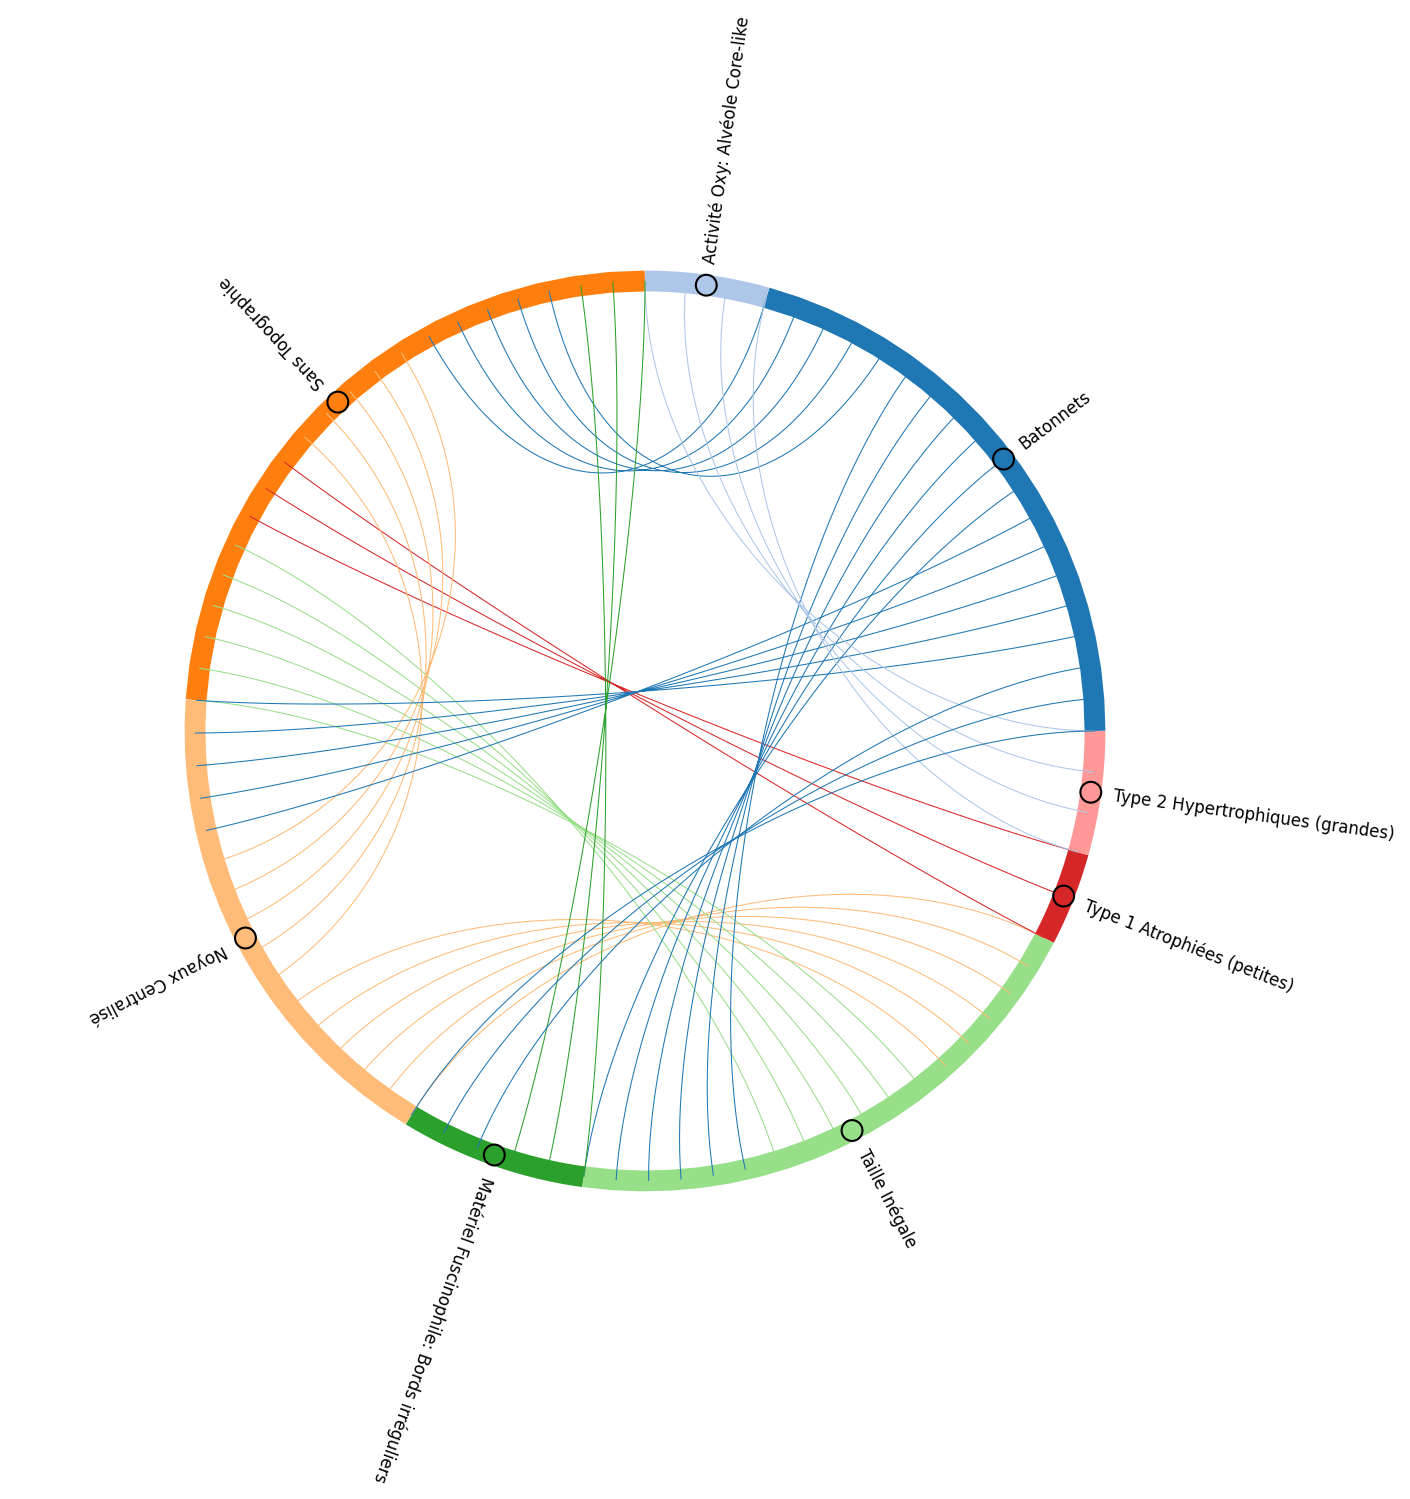
\includegraphics[width=1\textwidth]{figures/chord_plot.png}
  \caption[Diagramme de cordes des règles de LCS]{Diagramme de cordes des règles de LCS}
  \label{fig:chords}
\end{figure}
La seconde approche a permis de générer le réseau représenté dans la figure \ref{fig:network}. Cette figure est disponible de manière interactive à l'adresse \href{https://lbgi.fr/~meyer/myomap.html}{https://lbgi.fr/~meyer/myomap.html}. On observe sur cette représentation qu'une majorité des règles dans notre \gls{lcs} servent à essayer de différencier les \gls{cnm} du reste (de nombreux liens épais). Aussi, on observe que notre LCS essaie de différencier les \gls{cnm} principalement par l'absence de terme (majorité de liens rouges). Ces résultats supposent que l'algorithme parvient facilement à séparer les \gls{nm} des \gls{com} avec un faible jeu de règles, mais la tâche est plus compliquée pour les \gls{cnm}, pour lesquelles il génère un nombre important de règles. On retrouve sur ce réseau, des observations attendues comme la présence d'un lien vert entre \gls{nm} et le terme "bâtonnets", la présence d'un lien vert entre \gls{com} et le terme "cores", et la présence d'un lien vert entre \gls{cnm} et le terme "noyaux centralisés". On observe cependant aussi des critères de classification moins connus comme la présence de bords arrondis pour les fibre musculaire lié de façon positive au diagnostic \gls{cnm} et de façon négative au diagnostic \gls{nm}. Ou encore la présence d'anomalie de coloration PAS associée de façon positive aux \gls{nm} et négative aux \gls{cnm}. L'importance de la coloration PAS pour la classification a déjà été mise en évidence dans l'histogramme de l'importance des termes pour la classification présenté plus haut (fig. \ref{fig:feautre_importance}).
\begin{figure}[htbp]
  \centering
  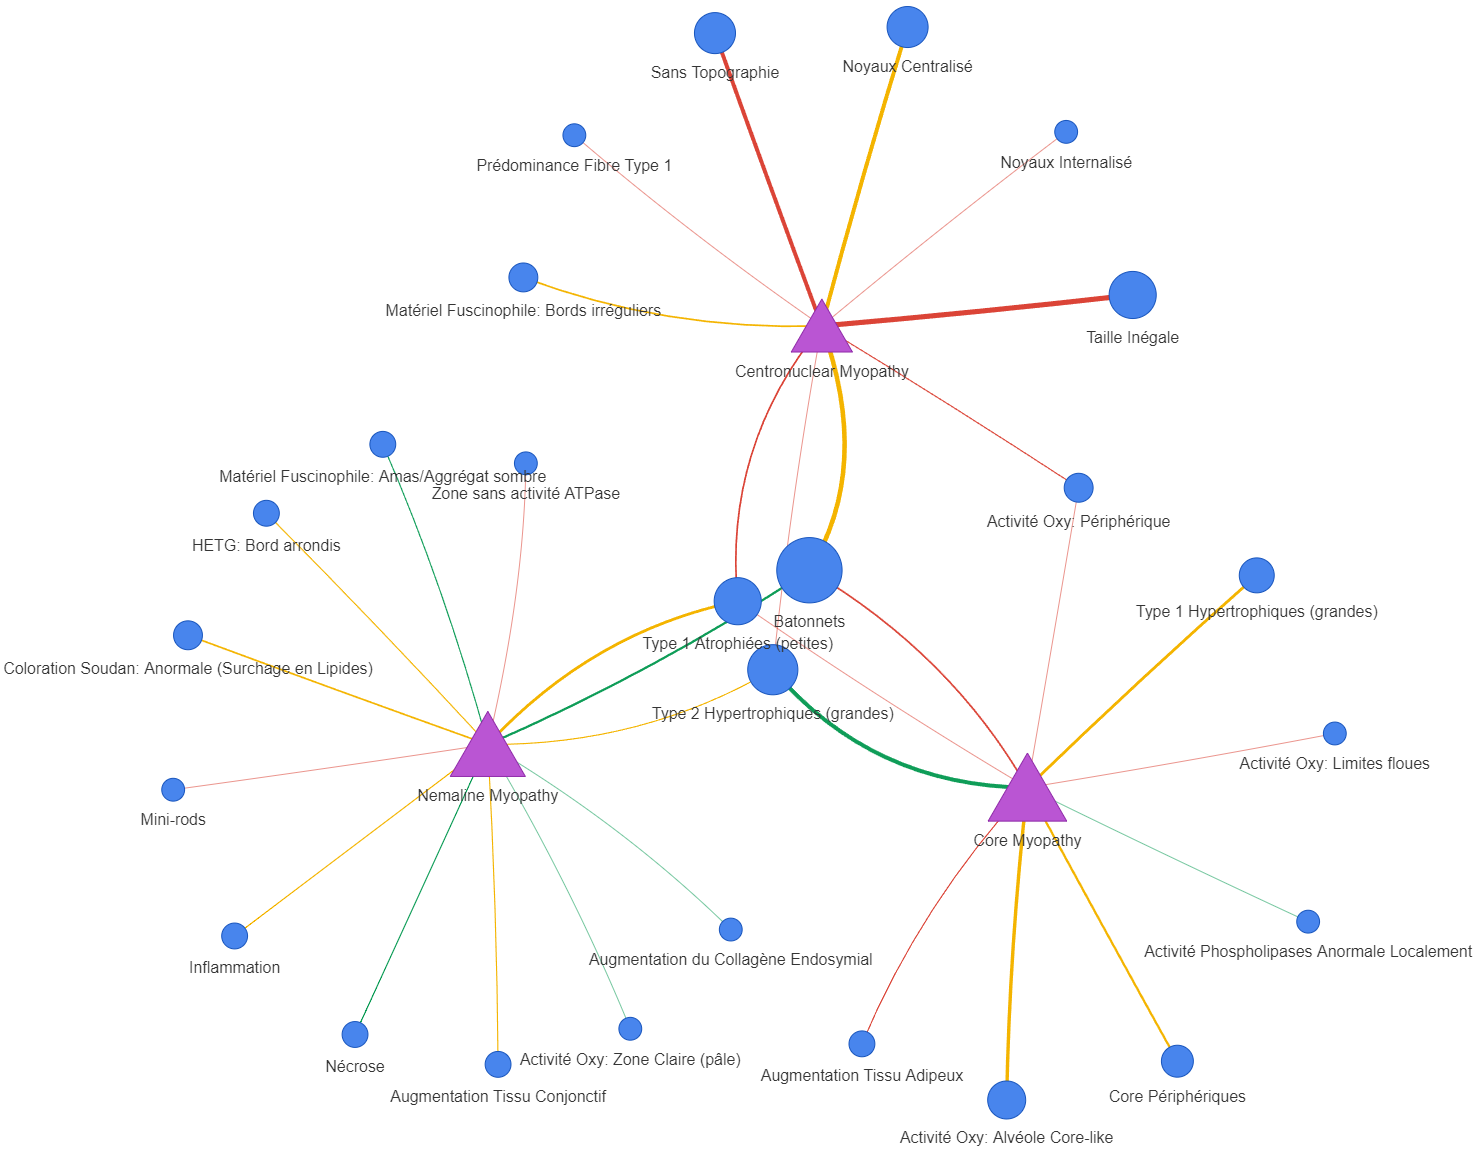
\includegraphics[width=1\textwidth]{figures/network_lcs.png}
  \caption[Représentation des règles de LCS sous forme de réseau]{Représentation des règles de LCS sous forme de réseau}
  \label{fig:network}
\end{figure}
\section{Perspectives de développement}
En terme développement futur, il est nécessaire d'agrandir le jeu de données utilisé pour comparer les algorithmes de classification. En effet, notre jeu de données de 89 rapports semble trop hétérogène et de trop petite taille pour déceler une différence de performances significative entre les algorithmes. De plus, il est nécessaire d'améliorer les approches de visualisation des règles de \gls{lcs}, car ces approches semblent être intéressantes pour visualiser graphiquement et rapidement le fonctionnement interne de notre système de classification explicable et pour identifier de nouveaux critères pertinent pour différencier les sous-types de myopathies congénitales.

Enfin il pourrait être intéressant d'intégrer ce pipeline d'entraînement et ces visualisations à \gls{impatient} pour entraîner automatiquement un modèle de classification performant lors de l'entrée de nouveaux patient. Ce modèle peut être mis à disposition ensuite dans le formulaire d'entrée pour réalise de l'aide au diagnostic.